\documentclass{book}
\usepackage[a4paper,
            left=0.5in,
            right=0.5in,
            top=0.5in,
            bottom=0.5in,
            ]{geometry}
\usepackage{minted}
\usepackage{graphicx}
\graphicspath{{.}}
\usepackage{adjustbox}
\usepackage{cprotect}
\setlength{\parindent}{0pt}
\begin{document}
{\Huge \textbf{Lab 4: Abstract Class and Interface}}
\\
\par
{
    \large
    \textbf{Objective:}
    \begin{itemize}
        \item{Understanding abstract methods and classes.}
        \item{Declare and implement Interface.}
    \end{itemize}
    \par
    \textbf{Programs:}
    \begin{enumerate}
        \item{Program to demonstrate the use of abstract class and interface to represent Shapes}
            \par
            \center{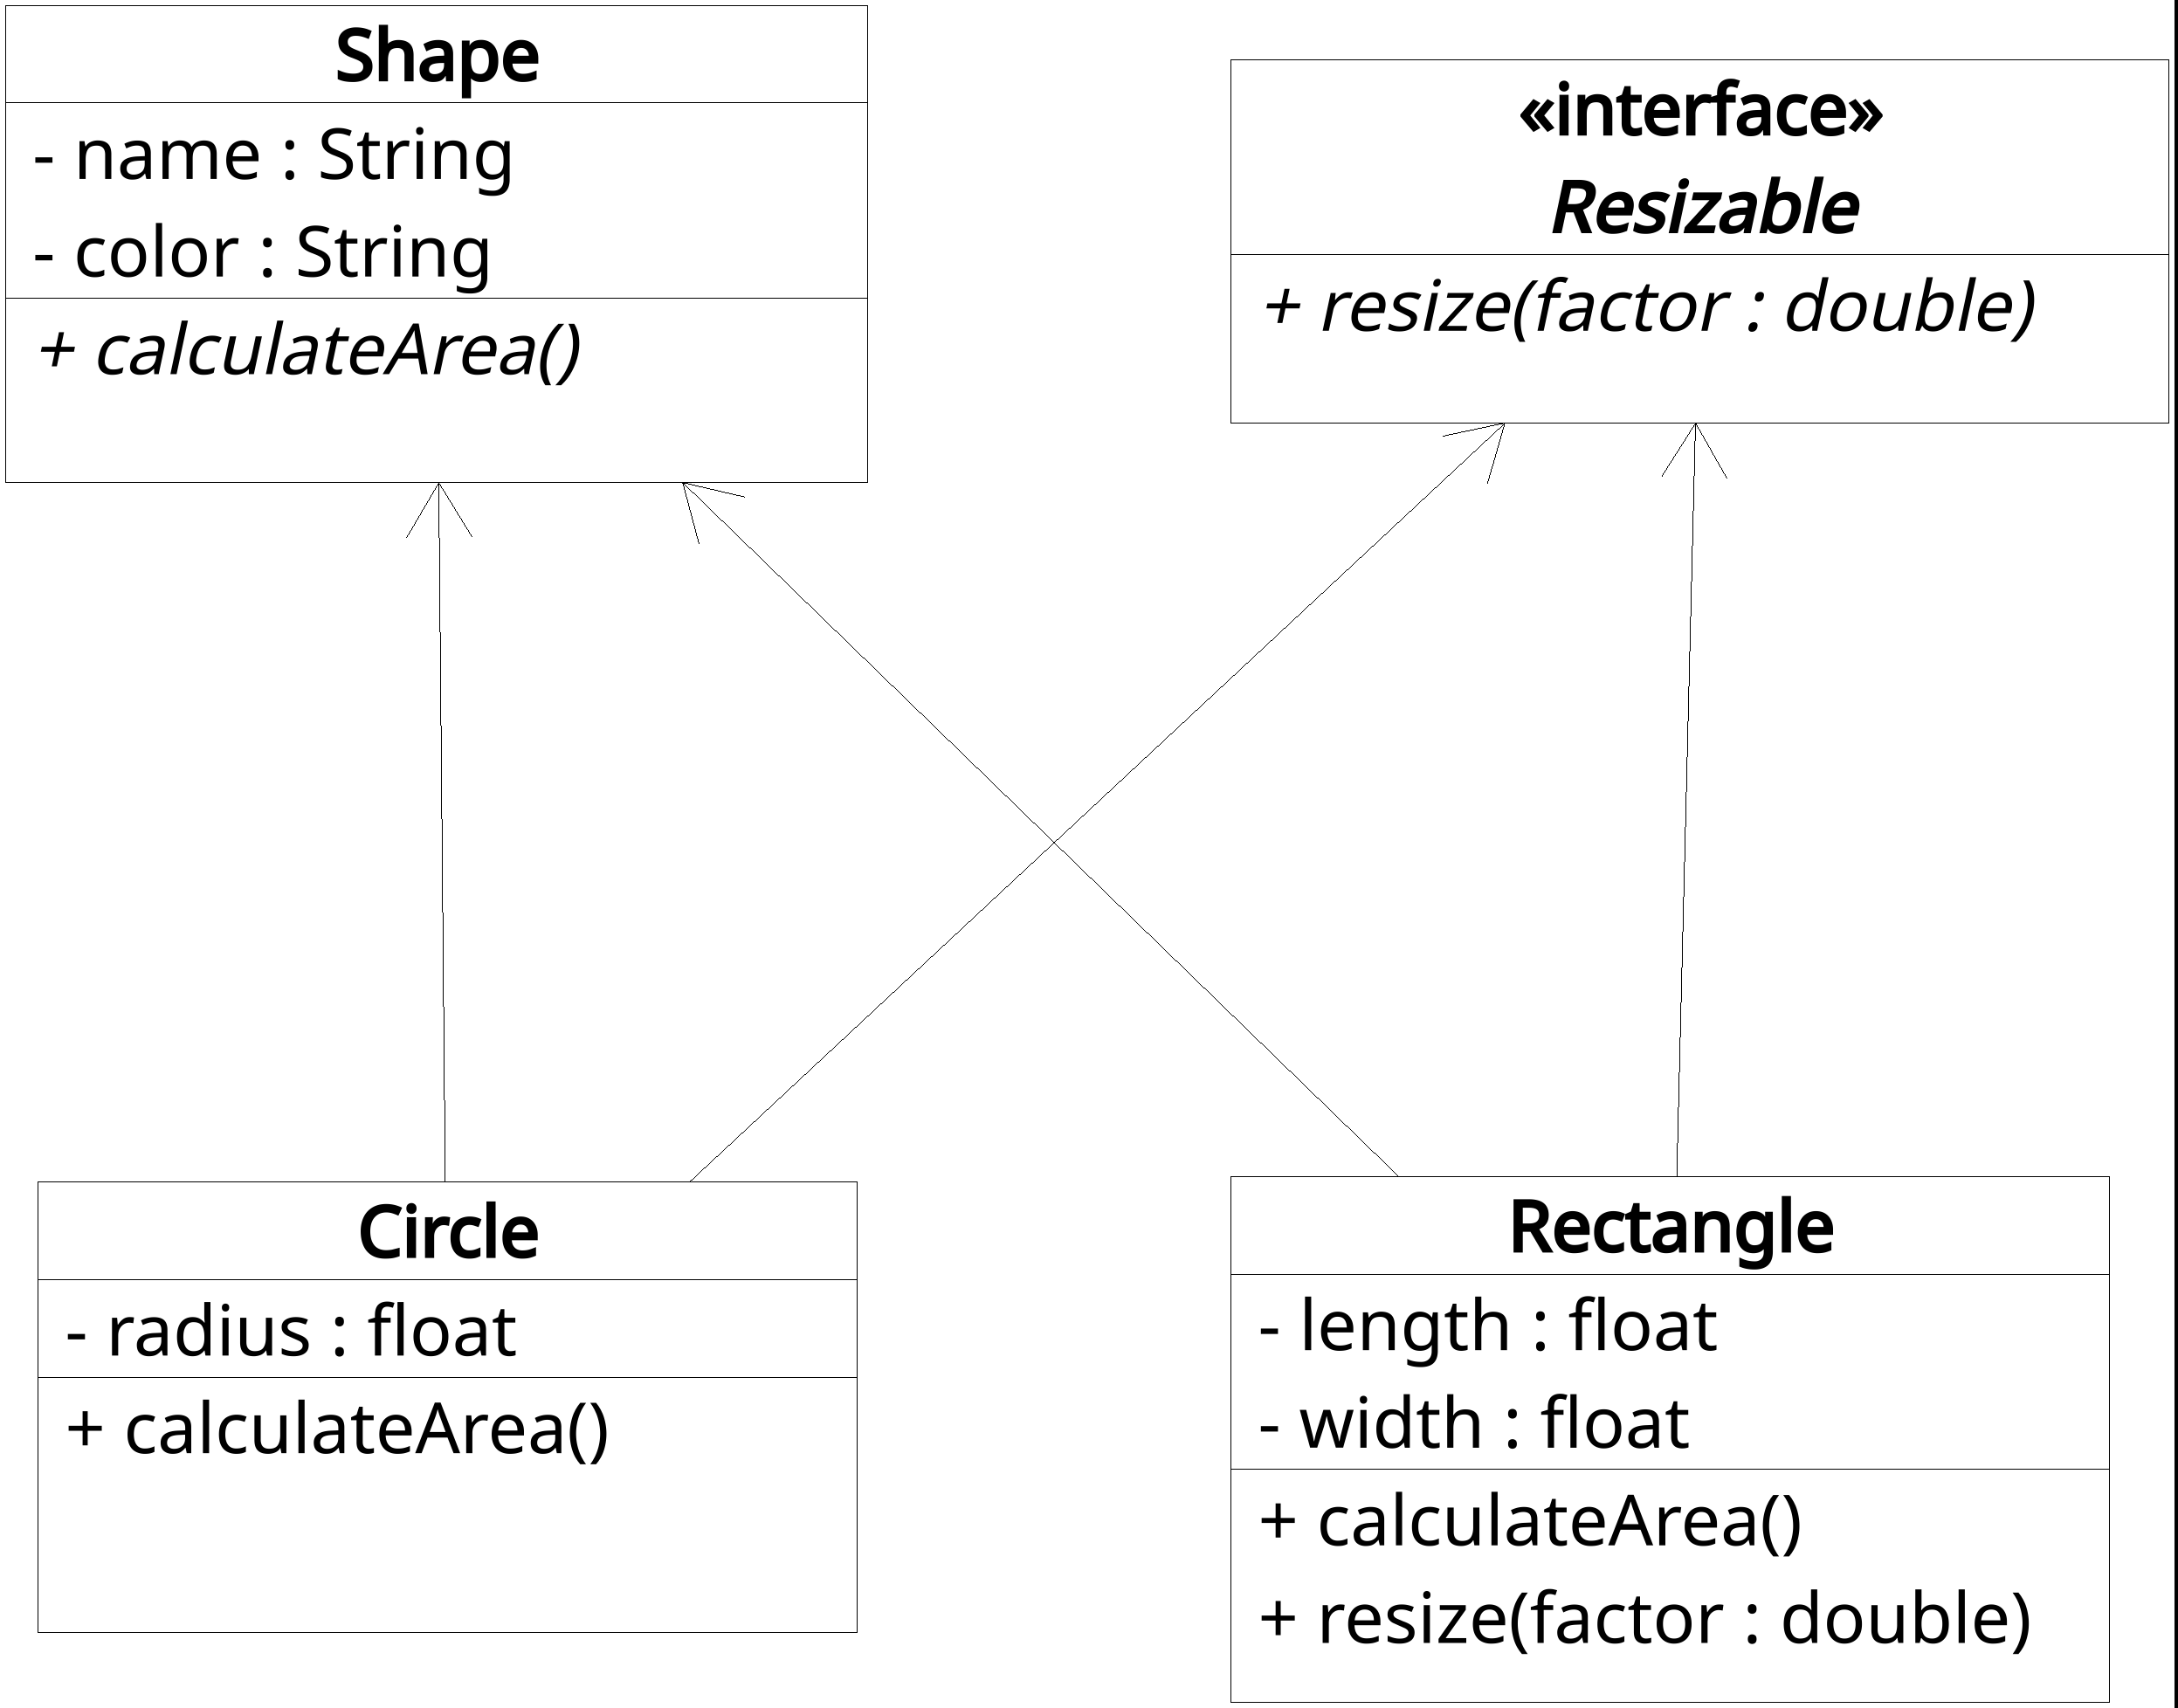
\includegraphics[width=0.8\textwidth,keepaspectratio]{shapeClassDiagram}}
            \begin{itemize}
                \item{/shapes/Shape.java}
                \inputminted{java}{shapes/Shape.java}
                \item{shapes/Circle.java}
                \inputminted{java}{shapes/Circle.java}
                \item{shapes/Rectangle.java}
                \inputminted{java}{shapes/Rectangle.java}
                \item{shapes/ResizeRectangle.java}
                \inputminted{java}{shapes/ResizeRectangle.java}
                \item{ShapeTest.java}
                \inputminted{java}{ShapeTest.java}
            \end{itemize}
            \par
            \textbf{Output:}
            \input{|"../output.sh ShapeTest"}
        \item{Program to demonstrate the use of abstract class and interface to represent Shapes}
            \par
            \center{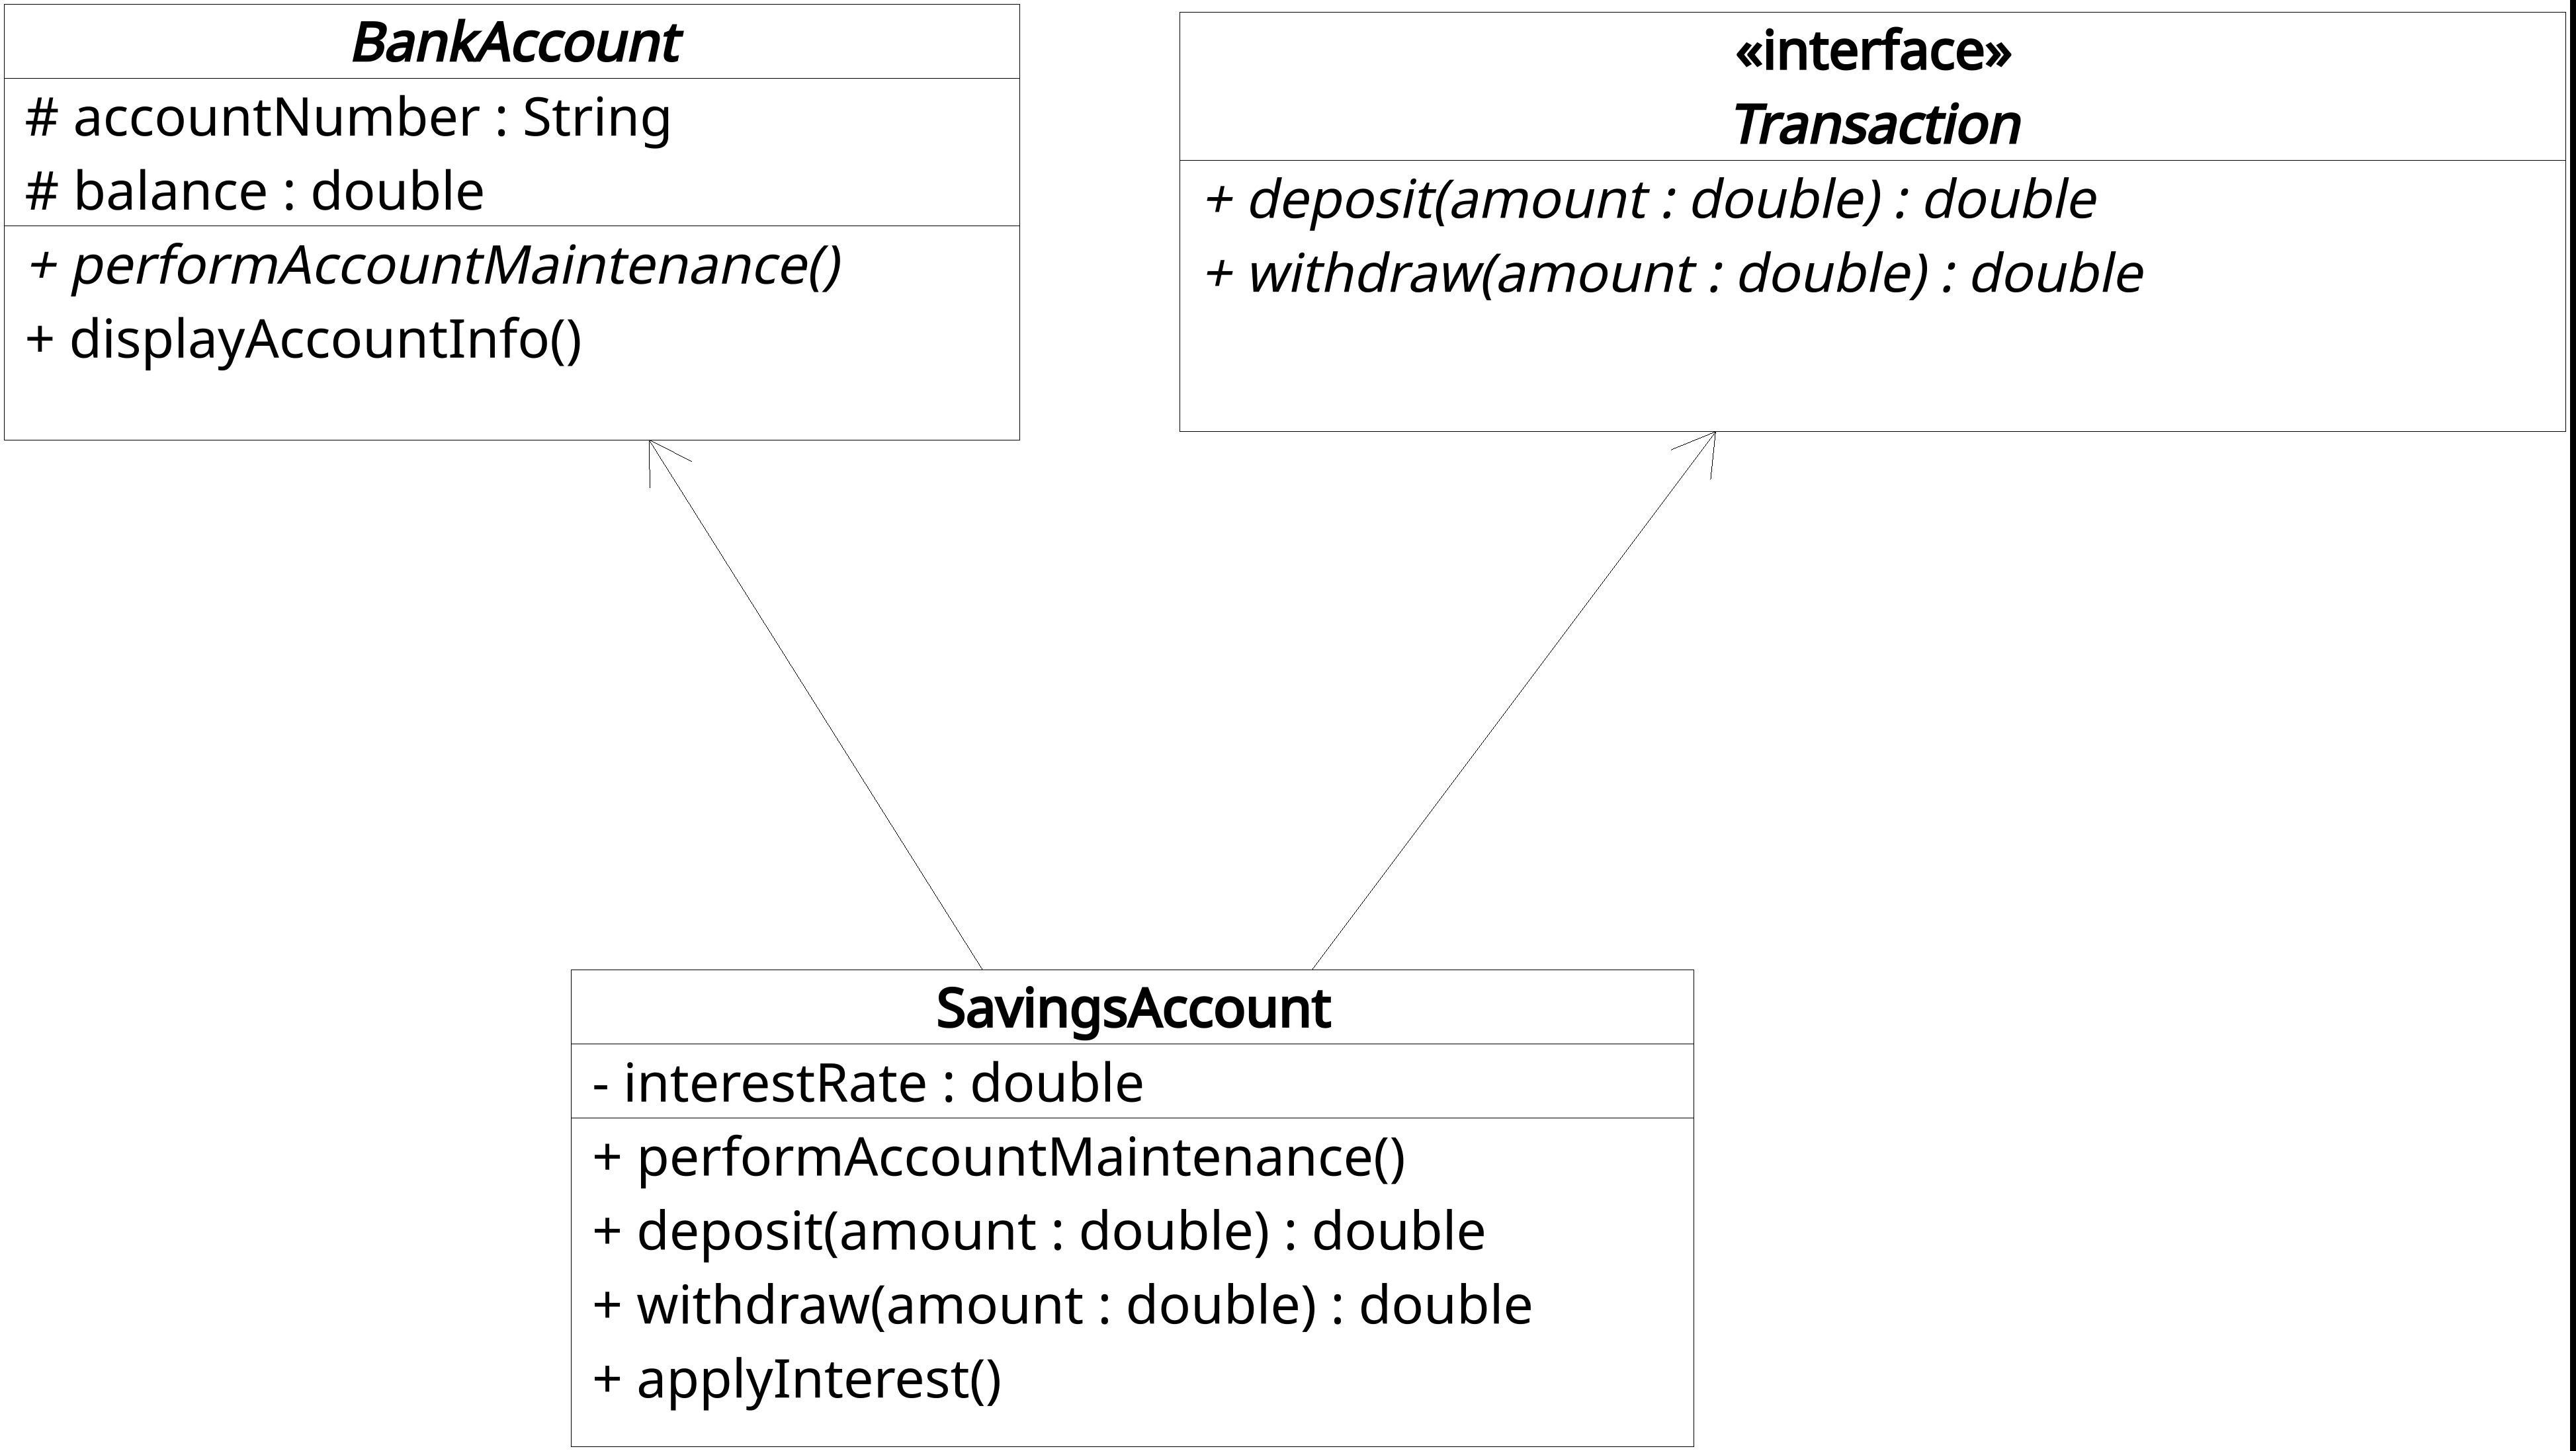
\includegraphics[width=0.8\textwidth,keepaspectratio]{bankClassDiagram}}
            \inputminted{java}{homework/BankingSystem.java}
            \par
            \textbf{Output:}
            \input{|"../output.sh homework/BankingSystem"}
    \end{enumerate}
    \par
    \textbf{Conclusion:}
    \begin{itemize}
        \item{We learned about abstract classes and methods.}
        \item{We learned about interfaces.}
    \end{itemize}
    
}

\end{document}
